\chapter*{Получение асимптотического решения на примере}
\addcontentsline{toc}{section}{Получение асимптотического решения на примере}

Получим асимптотическое решение $O(\varepsilon^2)$
в виде бегущей волны,
зависящей от $z=x-Vt$,
для возмущенного уравнения КдВ:
\begin{equation*}
    u_t + u u_x + b u_{xxx} = \varepsilon f(u),
\end{equation*}
где
\begin{equation*}
    f(u) = - a_1 u + a_2 u^2 - a_3 u^3
\end{equation*}

В соответствии с методами возмущений
решение задачи представляется
первыми двумя членами возмущённого разложения:
\begin{align}
    u(x, t, \varepsilon) & = u_0(x, t) + \varepsilon u_1(x, t) +
    O(\varepsilon^2) \nonumber \\
    u(x, t, \varepsilon) & \simeq u_0(x, t) + \varepsilon u_1(x, t). \label{Eq:u}
\end{align}

Для бегущей переменной $z = x - V t$
введём медленное время $T = \varepsilon t$,\\
тогда:
\begin{equation*}
    z = x - V(T) t % TODO перепроверить, непонятная запись
\end{equation*}

Операторы дифференцирования принимают вид:
\begin{align}
    \partial_x = \partial_z & =  
    \pdv{z}{x} \partial_z + \pdv{T}{x} \partial_T \\
    \partial_t & = \pdv{u}{t} =
    \pdv{z}{t} \partial_z + \pdv{T}{t} \partial_T =
    -V \partial_z + \varepsilon \partial_t
\end{align}

Обозначим за $F$ исходное уравнение:
\begin{equation} \label{Eq:F}
    F = u_t + u u_x + b u_{xxx} - \varepsilon f(u) = 0 
\end{equation}

Тогда после подстановки описанных выше преобразований получим:
\begin{equation*}
    F(u, u_z, u_{zzz}, T, \varepsilon) =
    -V(T) u_z + \varepsilon u_T + u u_z + b u_{zzz} +
    \varepsilon (a_1 u - a_2 u^2 + a_3 u^3) = 0
\end{equation*}

Подставим решение \eqref{Eq:u} в \eqref{Eq:F}
и сгруппируем коэффициенты при степенях $\varepsilon$.
% TODO опасная зона, нужно разбираться
Так как коэффициенты степеней обращаются в 0 независимо,
можно решить систему из двух уравнений:

\begin{equation} \label{Eq:system}
    \left\{ \,
    \begin{IEEEeqnarraybox}[][c]{l?s}
        \IEEEstrut
            F(u_0) = 0 & для $\varepsilon^0$ \\
            L u_1 = f(u_0) & для $\varepsilon^1$,
        \IEEEstrut
    \end{IEEEeqnarraybox}
    \right.
\end{equation}

где $L = -V(T) \partial_z + b \partial_z^3$
--- линейный дифференциальный оператор.

Данная задача разрешима в следствие альтернативы Фредгольма,
требуется выполнение условия $f \perp \operatorname{Ker}L^*$.
\begin{equation*}
    \begin{gathered}
        \nu \in \operatorname{Ker}L^* \Rightarrow (f, \nu) = 0 \\
        (L \nu, w)_{L^2} = (\nu, L^* w)_{L^2} \\
        w \in C_0^\infty(R).
    \end{gathered}
\end{equation*}

Необходимо, чтобы $\Lim{k \rightarrow \infty} |u^k| = 0$.

\begin{equation*}
    \begin{gathered}
        \int \left(a u_0 \nu_z - V \nu_z + u_{0,z} \nu + b \nu_{zzz} \right) w dz = \\
        = \int \nu \left( -(a u_0 \nu)_z + V w_z - u_{0,z} w - b w_{zzz} \right) dz \\
        \nu \in \operatorname{Ker}L^* \Rightarrow L \nu = 0
    \end{gathered}
\end{equation*}

При степени $\varepsilon^0$ коэффициент
представляет из себя уравнение Кортевега --- де Фриза (КдВ).
Для $u_0$ можем взять известное решение:
\begin{equation*}
    u_0 = \alpha \cosh^{-2}(c + k z) 
\end{equation*}

Тогда
\begin{equation*}
    \begin{gathered}
        L^* u_0 = 0 \Rightarrow u_0 \in \operatorname{Ker}L^* \\
        (f, u_0) = 0
    \end{gathered}
\end{equation*}

Выразим неизвестные через параметр $k$
для уравнения при $\varepsilon^0$ из \eqref{Eq:system}:
\begin{equation*}
    \begin{gathered}
        a = 12 b k \\
        V = 4 b k^2
    \end{gathered}
\end{equation*}

Из условий $u_0 \in \operatorname{Ker}L^*$
и $(f, u_0) = 0$ получаем дифференциальное уравнение
для $k$ и решаем его. Так как это новый параметр,
то мы удовлетворяем альтернативе Фредгольма.

Для решения второго уравнения системы \eqref{Eq:system}
решим сначала его с нулевой правой частью, т.е.:
\begin{equation*}
    L u_1 = -V(T) \partial_z u_1 + b \partial_z^3 u_1 = 0
\end{equation*}

Выполним интегрирование по $\partial_z$:
\begin{equation*}
    -V(T) u_1 + b \partial_z^2 u_1 = 0
\end{equation*}

Поделим на $b \neq 0$ обе части:
\begin{equation*}
    -\frac{V(T)}{b} u_1 + \partial_z^2 u_1 = 0
\end{equation*}

Выпишем точное решение уравнения:
\begin{equation*}
    u_1 = C_1 \sinh(z \sqrt{ \left|\frac{V}{b}\right|} ) +
    C_2 \cosh(z \sqrt{ \left|\frac{V}{b}\right|})
\end{equation*}

Используем данное соотношение в качестве анзаца
для решения второго уравнения системы \eqref{Eq:system}.
Шаги решения аналогичны решению первого уравнения.

Вывод выполнялся в Wolfram Mathematica 10.4.1.

Было получено решение:
\begin{equation*}
    u = 12 b \cosh^{-2}(x - 4 b t) +
    \varepsilon \left[ 12 a_2 a_3 b^2 \cosh(\sqrt{\frac{1}{b}} (x - 3 t)) -
    6 a_2 a_3 b^2 \right],
\end{equation*}

что соответствует первым двум членам возмущённого разложения \eqref{Eq:u}.

Ниже приведены графики решения
при $b = 1, t = 1, a_2 = 1, a_3 = 1$.

Параметр $\varepsilon$ принимает 3 значения,
различающиеся на порядок (конкретное значение указано в подписи к рисункам).

Синей линией показан первый член разложения $u_0$,
коричневой --- первые два члена разложения $u \sim O(\varepsilon^2)$.

\begin{figure}[H]
    \centering
    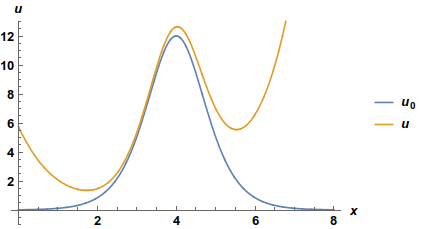
\includegraphics[width=\textwidth]{triv005}
    \caption{График решения при $\varepsilon = 0.05$}
\end{figure}
\begin{figure}[H]
    \centering
    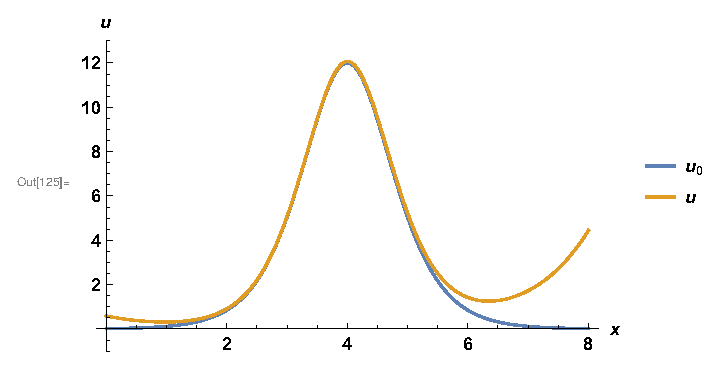
\includegraphics[width=\textwidth]{triv0005}
    \caption{График решения при $\varepsilon = 0.005$}
\end{figure}
\begin{figure}[H]
    \centering
    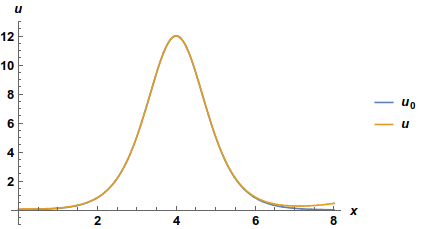
\includegraphics[width=\textwidth]{triv00005}
    \caption{График решения при $\varepsilon = 0.0005$}
\end{figure}

Из рисунков видно, что при $\varepsilon \to 0$
решение $u$ стремится к решению невозмущённого уравнения КдВ.

\section*{Выводы}
\addcontentsline{toc}{section}{Выводы}

Многие задачи прикладной математики, физики
и других областей не позволяют получить точные аналитические решения.
Для получения информации о решениях приходится обращаться к аппроксимации,
численным решениям или к их сочетанию.
Методы асимптотических разложений и
многих масштабов позволяют получить решения с приемлемой точностью.
